\documentclass[a4paper,12pt]{article}

\usepackage[backend=biber,style=numeric]{biblatex}
\addbibresource{references.bib}

\setlength{\parindent}{0pt}
\usepackage[utf8]{inputenc}
\usepackage[T1]{fontenc}
\usepackage[english,french]{babel}
\usepackage{graphicx}
\usepackage{amsmath,amssymb}
\usepackage{geometry}
\usepackage{titling}
\usepackage{hyperref}
\usepackage[ruled,vlined]{algorithm2e}
\geometry{a4paper, margin=1in}

\title{
  \Huge\textbf{Apprentissage de classes déséquilibrées}\\
  \LARGE HAX907X - Apprentissage statistique
}

\author{
EL SAWADOGO Kader\\
GERMAIN Marine\\
LABOURAIL Célia\\
MARIAC Damien
}

\date{\today}

\begin{document}

\maketitle

\begin{abstract}
Ce document présente le rapport du projet réalisé dans le cadre du cours d'apprentissage statistique. Il détaille les objectifs, la méthodologie, les résultats obtenus et les conclusions tirées.
\end{abstract}


\tableofcontents

\newpage

\section{Contexte et Objectifs}

Dans le cadre de ce travail, nous nous intéressons à l’apprentissage supervisé dans des contextes où les classes sont déséquilibrées.
Ce problème est fréquent dans de nombreux domaines, tels que la détection de fraudes, la médecine ou le diagnostic industriel. Un déséquilibre important des classes peut conduire à des modèles biaisés : ils tendent à prédire correctement les classes majoritaires en négligeant les classes minoritaires.\\

La problématique scientifique que nous étudions est donc la suivante : "Comment atténuer le déséquilibre de classes pour améliorer la performance des modèles ?"\\

L’objectif de ce travail est d’étudier des méthodes permettant de résoudre ce déséquilibre. Plus précisément, nous nous concentrons sur trois approches issues d’articles scientifiques :
\begin{enumerate}
    \item Le \textbf{Random Over-Sampling} (ROS) cité dans l’article \textit{Survey on Deep Learning with Class Imbalance} \cite{johnson2019survey}, une méthode de rééchantillonage qui consiste à augmenter artificiellement la proportion de la classe minoritaire.
    \item Le \textbf{Random Under-Sampling} (RUS), une autre méthode de rééchantillonage,  cité également dans l’article \cite{johnson2019survey} qui consiste à réduire la proportion de la classe majoritaire
    \item La \textbf{Synthetic Minority Over-sampling Technique} (SMOTE) présenté dans l’article \cite{chawla2002smote} qui génère de nouvelles instances synthétiques pour la classe minoritaire à partir des observations existantes
\end{enumerate}


\newpage

\section{Méthodologie Damien}

\newpage

\section{Forces et Faiblesses Célia}

\newpage

\section{Exemples d'applications Kader}

\newpage

\section{BRAIN STORM --------------------}

\section{Les différentes méthodes}
\subsection{Méthodes au niveau des données}
Les méthodes data-level agissent directement sur les données d’entraînement pour atténuer le
déséquilibre entre classes. Le principe est soit d’augmenter le poids de la classe minoritaire en lui
fournissant plus d’exemples (réels ou synthétiques), soit au contraire de réduire le poids de la classe
majoritaire en éliminant certains de ses exemples. L’objectif est d’obtenir une distribution de classes
plus équilibrée, ce qui force l’algorithme d’apprentissage à prêter autant d’attention à la minorité qu’à la
majorité. Ces techniques peuvent toutefois introduire de la variance (sur-apprentissage) ou du
biais supplémentaire, il faut donc les appliquer judicieusement.

\subsubsection{Sur-échantillonnage (Over-sampling)}

Le sur-échantillonnage (oversampling) consiste à ajouter des copies ou des variantes des exemples de
la classe minoritaire jusqu’à augmenter sa fréquence dans le jeu de données. Dans sa forme la plus
simple, le sur-échantillonnage aléatoire (Random Over-Sampling, ROS) duplique aléatoirement des
instances minoritaires existantes jusqu’à atteindre un équilibre désiré. Par exemple, si l’on dispose
de 100 exemples minoritaires et 1000 majoritaires, le ROS peut répliquer les minoritaires
(éventuellement plusieurs fois chacun) jusqu’à en obtenir 1000, rétablissant ainsi un ratio équilibré. On échantillonne avec remise parmi les indices de la classe minoritaire pour
générer de nouvelles instances d’entraînement.

\subsubsection{Sous-échantillonnage (Under-sampling)}

À l’inverse, le sous-échantillonnage (undersampling) vise à réduire la proportion de la classe
majoritaire en retirant certains de ses exemples du jeu de données. Le sous-échantillonnage aléatoire
(Random Under-Sampling, RUS) élimine au hasard des instances de la classe majoritaire jusqu’à atteindre
un ratio plus équilibré avec la minorité.le RUS est utile lorsque l’on dispose d’une grande abondance de
données majoritaires, potentiellement redondantes. Plutôt que de tout utiliser, ce qui peut être
coûteux et inutile, on peut se permettre d’en élaguer une partie. En réduisant drastiquement le nombre
d’exemples majoritaires, on élimine le biais numérique et on accélère l’entraînement (moins de
données à parcourir).

\subsubsection{SMOTE (Synthetic Minority Over-sampling Technique)}



Plutôt que de copier des instances existantes,
SMOTE crée de nouvelles instances minoritaires artificielles en interpolant entre des exemples réels.Concrètement, pour chaque exemple minoritaire original, SMOTE sélectionne aléatoirement l’un de ses
$k$ plus proches voisins (minoritaire également), puis génère un nouvel exemple situé aléatoirement le
long du segment joignant les deux points dans l’espace des \textit{features}. En répétant ce procédé, on
peut synthétiser autant d’exemples minoritaires que souhaité.



\subsection{Méthodes au niveau de l'algorithme }
????????
\newpage
\section{force et faiblesse }
Selon différents articles comme Bee Wah Yap et al. (2013), il est souvent préférable d’utiliser le Random Undersampling plutôt que le Random Oversampling, à condition que la taille du jeu de données le permette.
 En effet, le Random Oversampling consiste à dupliquer aléatoirement certaines observations de la classe minoritaire afin de rééquilibrer les classes. Cependant, cette duplication augmente le risque de surapprentissage (overfitting),
  car le modèle apprend alors trop précisément les exemples déjà présents dans la base de données, ce qui nuit à sa capacité à généraliser sur de nouvelles données.
Les méthodes classiques de rééchantillonnage présentent aussi certaines limites. Elles peuvent notamment conduire le modèle à croire que certaines combinaisons de variables expliquent à elles seules la majorité des observations minoritaires, ce qui peut fausser
 la compréhension réelle des relations entre variables.\medskip

 Contrairement à l’oversampling aléatoire, SMOTE ne duplique pas les données existantes mais crée de nouvelles observations synthétiques.  Cette approche permet d’enrichir la représentation de la classe minoritaire tout en limitant
  partiellement les risques d’overfitting.\medskip

Malgré ses avantages, SMOTE présente plusieurs inconvénients importants. Tout d’abord, son temps de calcul est plus long que celui des méthodes plus simples. Cela s’explique par le fait que l’algorithme doit calculer la distance
entre chaque observation minoritaire et tous les autres points pour identifier ses k plus proches voisins. Ce calcul devient rapidement coûteux lorsque la taille du jeu de données augmente, car le nombre de comparaisons croît de manière quadratique (de l’ordre de O(n²)). En pratique, cela signifie que sur des bases volumineuses ou avec beaucoup de variables, SMOTE peut nécessiter des temps de traitement bien plus élevés,
surtout lorsqu’il est utilisé à chaque étape d’une validation croisée.
Un autre problème souvent mentionné dans la littérature concerne la sensibilité de SMOTE aux points aberrants. Si une observation minoritaire isolée se trouve très proche d’un point appartenant à la classe majoritaire, l’algorithme risque d’utiliser cette proximité
pour créer de nouvelles données synthétiques incorrectes. Cela peut introduire du bruit et perturber l’apprentissage du modèle. Pour limiter ce problème, il est possible d’ignorer les observations minoritaires dont les k plus proches voisins appartiennent principalement
 à la classe majoritaire, afin d’éviter de générer des points non représentatifs.\medskip


Plusieurs variantes de SMOTE ont été développées pour corriger ces défauts.
Par exemple :
\begin{itemize}
    \item \textbf{SMOTE-NC (Nominal and Continuous)} : s’adapte aux jeux de données contenant à lafois des variables continues et qualitatives ;
    \item \textbf{Borderline-SMOTE} (Hui Han, Wen-Yuan Wang et Bing-Huan Mao, 2005 ) : se concentre sur les points situés à la frontière entre classes, considérés comme plus informatifs pour le modèle.
\end{itemize}

SMOTE représente une amélioration importante par rapportaux méthodes de rééchantillonnage aléatoires, car il permet de mieux exploiter l’information disponible dans la classe minoritaire. Toutefois, il reste plus coûteux en calcul et sensible aux valeurs aberrantes, ce qui peut poser problème lorsque la base de donnée est très volumineuse ou lorsque les ressources de calcul sont limitées. Le choix de la méthode de rééchantillonnage doit donc se faire en tenant compte à la fois de la taille des données, du type de variable et du temps de traitement disponible.

\bigskip
\textbf{Source :} MÉTHODES DE RÉÉQUILIBRAGE DES CLASSES en classification supervisée, Merwan CHELOUAH.



\newpage

\section*{Méthodes de gestion du déséquilibre des classes}

\subsection*{Algorithme 1 : Full Data (sans rééquilibrage)}
\begin{algorithm}[H]
\caption{Full Data (sans rééquilibrage)}
\KwIn{Dataset $D$ avec classes $C_{maj}$ et $C_{min}$}
\KwOut{Dataset inchangé $D'$}

Séparer $D$ en train et test\;
Standardiser les variables\;
\Return $D'$\;
\end{algorithm}

\subsection*{Algorithme 2 : Random Undersampling}
\begin{algorithm}[H]
\caption{Random Undersampling}
\KwIn{Dataset $D$ avec classes $C_{maj}$ et $C_{min}$}
\KwOut{Dataset équilibré $D'$}

$n_{min} \gets |C_{min}|$ \;
Sélectionner aléatoirement $n_{min}$ échantillons de $C_{maj}$\;
Construire $D' = C_{min} \cup$ sous-échantillon($C_{maj}$)\;
\Return $D'$\;
\end{algorithm}

\subsection*{Algorithme 3 : Random Oversampling}
\begin{algorithm}[H]
\caption{Random Oversampling}
\KwIn{Dataset $D$ avec classes $C_{maj}$ et $C_{min}$}
\KwOut{Dataset équilibré $D'$}

$n_{maj} \gets |C_{maj}|$ \;
\While{$|C_{min}| < n_{maj}$}{
   Dupliquer aléatoirement un échantillon de $C_{min}$\;
}
Construire $D' = C_{maj} \cup C_{min}$ (après duplication)\;
\Return $D'$\;
\end{algorithm}

\subsection*{Algorithme 4 : SMOTE}
\begin{algorithm}[H]
\caption{Borderline-SMOTE (Synthetic Minority Oversampling Technique)}
\KwIn{Dataset $D$ avec classes $C_{maj}$ et $C_{min}$, nombre de voisins $k$}
\KwOut{Dataset équilibré $D'$}

\ForEach{$x_i \in C_{min}$}{
   Trouver les $k$ plus proches voisins de $x_i$ dans $D$\;
   \uIf{tous les voisins appartiennent à $C_{maj}$}{
      Marquer $x_i$ comme \textbf{bruit} (non utilisé)\;
   }
   \uElseIf{la majorité des voisins appartiennent à $C_{maj}$}{
      Marquer $x_i$ comme \textbf{danger}\;
   }
   \Else{
      Marquer $x_i$ comme \textbf{safe} (non utilisé)\;
   }
}

\ForEach{$x_i$ marqué comme \textbf{danger}}{
   Sélectionner aléatoirement un voisin minoritaire $x_{voisin}$ parmi ses $k$ plus proches voisins\;
   Générer un nombre aléatoire $\lambda \sim U(0,1)$\;
   Créer un point synthétique :
   \[
      x_{\text{new}} = x_i + \lambda \cdot (x_{voisin} - x_i)
   \]
   Ajouter $x_{\text{new}}$ à $C_{min}$\;
}

Construire $D' = C_{maj} \cup C_{min}$ (avec points synthétiques générés)\;
\Return $D'$\;
\end{algorithm}


\subsection*{Étape finale commune}
\begin{algorithm}[H]
\caption{Application de la régression logistique et évaluation}
\KwIn{Dataset équilibré $D'$ obtenu par Full Data, Undersampling, Oversampling ou SMOTE}
\KwOut{Performance du modèle}

Diviser $D'$ en données d'apprentissage (train) et de test (test)\;
Standardiser les variables explicatives\;
Entraîner une \textbf{régression logistique} sur l'échantillon d'apprentissage\;
Prédire les probabilités sur l'échantillon test\;
Tracer la \textbf{courbe ROC} et calculer l'\textbf{AUC}\;
Construire la \textbf{matrice de confusion} pour évaluer les performances\;
\Return{ROC, AUC, matrice de confusion}\;
\end{algorithm}



\section{Exemple d'application : Détection de fraudes par carte bancaire}

L’objectif de cette application est de mettre en place un modèle de détection de fraudes à partir du jeu de données \textit{Credit Card Fraud Detection} disponible sur Kaggle.
Ce jeu contient 284\,807 transactions, dont seulement 492 sont frauduleuses (soit environ 0,17 \%).
Le fort déséquilibre entre les classes rend la tâche difficile, car un modèle naïf qui prédirait toujours ``non fraude'' atteindrait déjà une précision (accuracy) proche de 99,8 \%.
Pour dépasser cette limite, plusieurs stratégies de gestion du déséquilibre ont été appliquées et comparées en utilisant une régression logistique.

\subsection*{Régression logistique sans traitement}
Dans un premier temps, nous avons entraîné le modèle sur l’ensemble complet, sans traitement particulier du déséquilibre.
Les résultats montrent une accuracy très élevée (0,9991), mais trompeuse, puisque le rappel (sensitivity) des fraudes n’est que de 0,61.
Autrement dit, la majorité des fraudes ne sont pas détectées, ce qui rend le modèle inutilisable en pratique malgré une performance apparente.

\subsection*{Random undersampling}
Afin de corriger ce problème, nous avons testé le \textit{random undersampling}, qui consiste à équilibrer les classes en réduisant volontairement le nombre de transactions normales pour égaler celui des fraudes.
Dans ce cas, le modèle obtient une \textit{balanced accuracy} d’environ 0,956 avec un rappel de 0,959.
Le modèle apprend donc à bien reconnaître les fraudes, mais au prix d’une perte importante d’information, puisque la majorité des transactions légitimes est écartée.

\subsection*{Random oversampling}
La seconde approche est le \textit{random oversampling}, qui duplique aléatoirement les fraudes afin de créer un jeu équilibré.
Cette méthode conserve toutes les données disponibles et améliore le rappel (0,977), ce qui signifie que presque toutes les fraudes sont détectées.
La \textit{balanced accuracy} atteint 0,949.
Toutefois, l’inconvénient de cette méthode est le risque de surapprentissage, car les exemples de fraude sont répétés artificiellement sans ajouter de diversité.

\subsection*{SMOTE}
Enfin, nous avons appliqué la méthode \textit{SMOTE (Synthetic Minority Oversampling Technique)}, qui génère artificiellement de nouveaux exemples de fraude en interpolant entre des observations existantes.
Cette méthode dépasse les performances des précédentes, avec une accuracy globale de 0,981, un rappel de 0,992 et une spécificité de 0,970.
Elle offre donc le meilleur compromis entre la détection des fraudes et la limitation des faux positifs.



\newpage

\section*{Annexe}

\begin{figure}[h!]
    \centering
    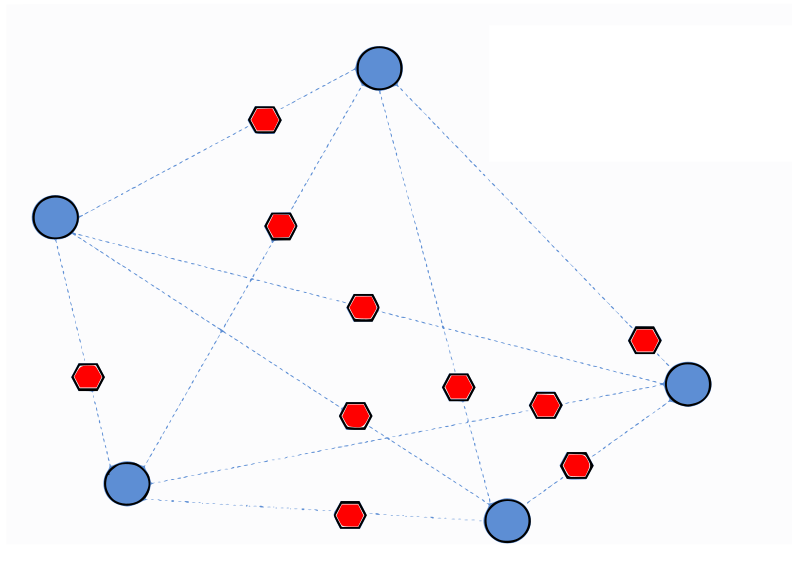
\includegraphics[width=0.8\textwidth]{images/smote.png}
    \caption{Smote illustration}
    \label{fig:example}
\end{figure}
Les points bleu correspondent à la classe minoritaire dont on souhaite générer de nouveaux exemples, les points rouge sont les points générés par SMOTE.

\newpage

\printbibliography

\end{document}